\secnumbersection{MARCO CONCEPTUAL}\label{ch:marco}

Para establecer correctamente los alcances de esta investigación es necesario conocer los fundamentos teóricos y físicos de las diferentes disciplinas involucradas. Es por esto que en este capítulo se exponen los principios de la hemodinámica vascular y su adquisición mediante \textit{4D Flow MRI}. Posteriormente, se analiza la base física del ultrasonido Doppler, cuyo modelo espectral es el estándar a emular, seguido de los conceptos de procesamiento digital de señales y mapeo de parámetros que fundamentan la técnica de sonificación. Finalmente, se presenta el estado del arte, donde se examinan aplicaciones de la síntesis acústica en el entorno clínico, estableciendo antecedentes que fundamentan la propuesta de extrapolar la sonificación al dominio del \textit{4D Flow MRI}.

\subsection{Hemodinámica vascular}\label{sec:hemodinamica}

La hemodinámica es la rama de la biofísica que estudia el comportamiento del flujo sanguíneo a través del sistema cardiovascular \cite{Roach1977}. Para modelar matemáticamente este comportamiento, la sangre suele aproximarse como un fluido incompresible y newtoniano en los vasos de gran y mediano calibre, asumiendo que su viscosidad se mantiene constante independientemente del gradiente de velocidad (tasa de cizalladura).

En tramos rectos y en condiciones fisiológicas normales, el flujo sanguíneo adopta un régimen laminar. Bajo estas condiciones, el fluido se desplaza en capas cilíndricas concéntricas que se deslizan unas sobre otras sin mezclarse de forma lateral \cite{klabunde_laminar}. Debido a la fricción con la pared vascular, la velocidad de la sangre es nula en los bordes (\textit{no-slip condition}) y alcanza su magnitud máxima en el eje central del vaso. Este comportamiento origina un perfil de velocidades parabólico, cuyo campo de velocidades puede ser descrito de forma idealizada mediante la ley de \textit{Poiseuille} \cite{Connes2025}.

El comportamiento ideal del flujo sanguíneo queda ilustrado en la Figura \ref{fig:flujo_laminar}:

\begin{figure}[H]
    \centering
    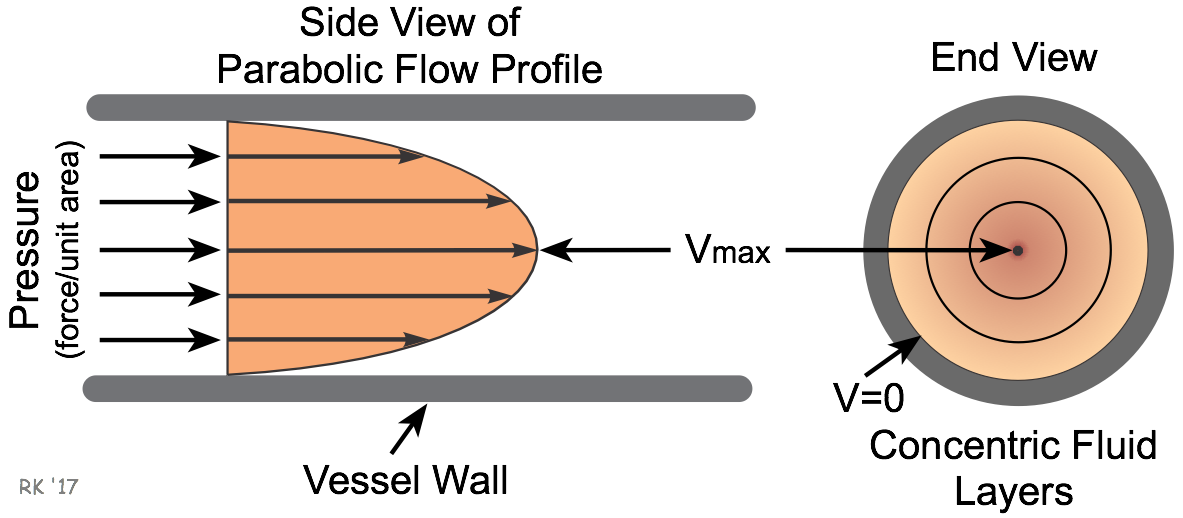
\includegraphics[width=0.7\textwidth]{figures/marco/laminar_flow.png}
    \caption{Perfil de flujo parabólico idealizado, donde la velocidad es máxima en el centro y nula en las paredes. Fuente: Tomado de \cite{klabunde_laminar}.}
    \label{fig:flujo_laminar}
\end{figure}

No obstante, el flujo sanguíneo \textit{in vivo} rara vez es estacionario, ya que su naturaleza es inherentemente pulsátil. Este fenómeno está dictado por las fases de contracción y relajación del ciclo cardíaco (sístole y diástole). Junto con la pulsatilidad, también se incorpora la compleja geometría del árbol vascular (curvaturas y bifurcaciones), generando campos de velocidades complejos que varían dinámicamente en el tiempo \cite{Ku1997}.

Capturar íntegramente esta distribución espacial de velocidades y su naturaleza pulsátil es una condición estricta, ya que esto permitirá el correcto desarrollo de algoritmos de síntesis espectral y sonificación.

\subsection{Adquisición mediante \textit{4D Flow MRI}}

La técnica \textit{4D Flow MRI} se ha consolidado como una herramienta fundamental para capturar la complejidad del flujo sanguíneo. Esta modalidad es una extensión volumétrica y temporal de la técnica convencional de resonancia magnética de contraste de fase (\textit{PC-MRI}, por sus siglas en inglés) \cite{markl2012_4dflow}.

Desde un punto de vista práctico, la base de esta modalidad se sustenta en que los protones en movimiento dentro del torrente sanguíneo experimentan un cambio en la fase de la señal de resonancia, el cual es directamente proporcional a su velocidad espacial. Para cuantificar este desplazamiento sin errores, el parámetro de adquisición más crítico es la codificación de velocidad o VENC (\textit{Velocity Encoding}). Este se define como la velocidad máxima (ya sea positiva o negativa) que puede ser registrada sin errores \cite{pineda2016_4dflow}. Si la velocidad real del flujo sanguíneo supera el VENC preestablecido, se produce un artefacto de ambigüedad conocido como \textit{aliasing} o solapamiento, el cual invierte artificialmente la dirección registrada del flujo y corrompe los datos cinemáticos. En los casos donde las velocidades fisiológicas superan el VENC configurado, es necesario repetir la adquisición con un valor mayor o aplicar técnicas de posprocesamiento para la corrección de fase (\textit{phase unwrapping}). Por consiguiente, resulta indispensable estimar a priori la velocidad máxima del vaso a estudiar para configurar adecuadamente este parámetro.

El concepto de ``cuatro dimensiones'' en la técnica \textit{4D Flow MRI} se deriva de la captura simultánea de tres dimensiones espaciales y una temporal. A diferencia del \textit{PC-MRI} bidimensional que evalúa el flujo en un único plano, esta modalidad codifica los vectores de velocidad en las tres direcciones ortogonales del espacio ($v_x, v_y, v_z$). Simultáneamente, la dimensión temporal se obtiene sincronizando la adquisición con el ciclo cardíaco del paciente mediante el electrocardiograma (ECG). Este acoplamiento divide el ciclo en múltiples intervalos temporales, permitiendo reconstruir la dinámica del flujo tridimensional a lo largo de un latido promedio representativo \cite{pineda2016_4dflow,markl2012_4dflow}.

El resultado final de este proceso es un vasto conjunto de datos discretos compuesto por tres dimensiones espaciales y una dimensión temporal. En cada vóxel (\textit{volumetric pixel}) del dominio tridimensional y para cada instante de tiempo del ciclo cardíaco, se registra la magnitud anatómica y un vector de velocidad espacial tridimensional.

Previo a cualquier análisis computacional, este volumen de datos brutos requiere una etapa de posprocesamiento mediante segmentación vascular \cite{Soulat2020}. El objetivo de este paso es aislar el vaso de interés del resto de los tejidos estáticos capturados durante la resonancia. Esto asegura que la matriz de velocidades resultante contenga exclusivamente la información hemodinámica del vaso deseado. Con este dominio aislado, los datos quedan habilitados para generar representaciones visuales tridimensionales y realizar cálculos cuantitativos sobre el flujo.

\subsection{Ultrasonido Doppler}\label{subsection:doppler_ultrasound}

El ultrasonido Doppler es una técnica de imagenología que permite evaluar la velocidad del flujo sanguíneo de forma no invasiva. Su funcionamiento se fundamenta en el efecto Doppler, un fenómeno físico caracterizado por el cambio en la frecuencia percibida de una onda cuando existe un movimiento relativo entre la fuente emisora y el receptor. En el contexto hemodinámico, un transductor piezoeléctrico emite pulsos acústicos a una frecuencia fundamental ($f_0$) hacia el interior del vaso sanguíneo. Los glóbulos rojos en movimiento actúan como partículas dispersoras (\textit{scatterers}) que reflejan estas ondas de vuelta hacia el transductor con una frecuencia alterada \cite{Poggi2024}.

La diferencia entre la frecuencia emitida y la frecuencia recibida se conoce como \textit{Doppler shift} ($f_d$) y es directamente proporcional a la velocidad de la sangre. Esta relación matemática se expresa mediante la ecuación clásica de Doppler (\ref{eq:doppler_clasica}) \cite{GOFFI2025217}:

\begin{equation}
    f_d = \frac{2 f_0 v \cos(\theta)}{c}
    \label{eq:doppler_clasica}
\end{equation}

Donde $v$ corresponde a la velocidad del flujo, $c$ representa la velocidad de propagación del sonido en los tejidos blandos, y $\theta$ es el ángulo de insonación, es decir, el ángulo formado entre el haz de ultrasonido incidente y el vector de dirección del flujo sanguíneo. La ecuación (\ref{eq:doppler_clasica}) puede ser reescrita para calcular la velocidad del flujo tal como se muestra en la ecuación (\ref{eq:velocidad_doppler}):

\begin{equation}
     v = \frac{c f_d}{2 f_0 \cos(\theta)} 
    \label{eq:velocidad_doppler}
\end{equation}

Como se estableció en \ref{sec:hemodinamica}, el flujo sanguíneo no presenta una velocidad única y homogénea, sino que se distribuye de manera parabólica y pulsa a lo largo del tiempo. Por consiguiente, el haz de ultrasonido no registra un único desplazamiento en la frecuencia, sino un espectro continuo de frecuencias superpuestas provenientes de las distintas capas del fluido. Esta multiplicidad de ecos acústicos genera lo que se conoce en el procesamiento de señales como ensanchamiento espectral (\textit{spectral broadening}) \cite{GOFFI2025217}.

Una visualización de este fenómeno se puede observar en la Figura \ref{fig:doppler_shift}, la cual expone una representación espectral donde se grafican las velocidades del flujo sanguíneo en función del tiempo.
 
\begin{figure}[H]
    \centering
    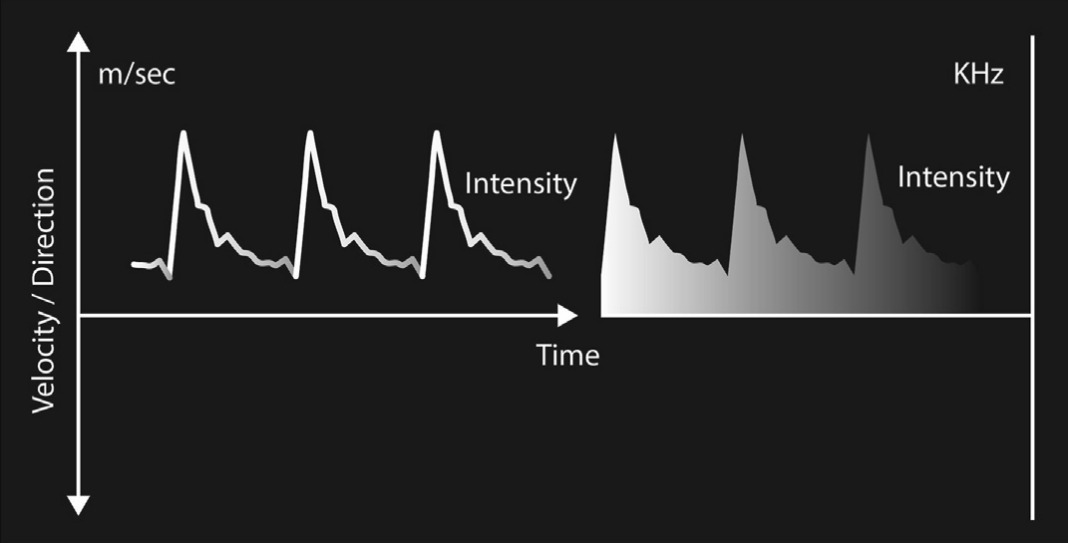
\includegraphics[width=0.7\textwidth]{figures/marco/doppler_shift.jpeg}
    \caption{Representación esquemática del desplazamiento de frecuencia (\textit{Doppler shift}) originado por los glóbulos rojos en movimiento. Fuente: Tomado de \cite{GOFFI2025217}.}
    \label{fig:doppler_shift}
\end{figure}

Una de las modalidades del ultrasonido Doppler que aplica el \textit{Doppler shift} es el \textit{Pulsed Wave Doppler} (\textit{PW-Doppler}). Esta modalidad otorga una resolución espacial, permitiendo definir una región de interés (\textit{ROI} por sus siglas en inglés) o volumen de muestra (\textit{sample volume}) a una profundidad y tamaño específico dentro del vaso sanguíneo. Al posicionar este volumen de muestra sobre el área a evaluar, el sistema es capaz de capturar los diferentes desplazamientos de frecuencia generados por los glóbulos rojos que atraviesan esta delimitación espacial. Dado que el volumen de muestra suele abarcar una región con múltiples velocidades, la señal resultante contiene el ensanchamiento espectral previamente descrito \cite{Oglat2018,GOFFI2025217}.

Para interpretar la superposición de ecos provenientes de la ROI, los sistemas de ultrasonido procesan la señal mediante análisis espectral, empleando clásicamente la Transformada Rápida de Fourier (\textit{FFT}). Este procesamiento matemático se traduce en dos salidas simultáneas: una representación gráfica continua conocida como espectrograma Doppler, y una salida acústica. Esta última ocurre de manera inherente, dado que las frecuencias del \textit{Doppler shift} fisiológico suelen coincidir con el rango de audición humana (típicamente entre 100 Hz y 8 kHz). De este modo, la señal procesada actúa como una sonificación natural que proporciona retroalimentación auditiva en tiempo real, permitiendo identificar características hemodinámicas como la pulsatilidad o la turbulencia a través del sonido \cite{hermann2011sonification}.


\subsection{Procesamiento digital de señales y mapeo de parámetros}

El procesamiento digital de señales (PDS) comprende el análisis, modificación y síntesis de señales representadas en formato discreto. En el ámbito del audio computacional, el PDS proporciona las herramientas matemáticas y algorítmicas necesarias para generar y manipular ondas sonoras a través de operaciones como la generación de osciladores, el filtrado, la modulación y la síntesis espectral \cite{dePoli1983,Moorer1977}.

Previo a la síntesis de audio es necesario que los datos hemodinámicos sean correctamente discretizados. Una forma de modelar la hemodinámica en segmentos específico de un una región vascular, es utilizando una estimación geométrica de la trayectoria principal del vaso, conocida como eje central o \textit{centerline} \cite{Antiga2008}. La extracción y visualización de las velocidades a lo largo de este \textit{centerline} permite establecer un sistema de referencia local. Evaluar planos transversales perpendiculares a este eje, permite extraer matrices que contienen la magnitud y dirección de las diferentes velocidades en cada porción del vaso. Estos son valores de entrada fundamentales para los diferentes algoritmos de PDS.

\subsubsection{Oscilador digital e integración de fase}\label{subsection:integracion_fase}

En el ámbito del procesamiento digital de señales, la generación sintética de sonido se realiza mediante osciladores digitales \cite{tierney1971digital}. Un oscilador básico produce una forma de onda periódica, siendo la onda senoidal la unidad armónica más simple. La representación matemática en tiempo discreto de una señal senoidal $s(n)$ está dada por la ecuación (\ref{eq:senoidal_discreto}):

\begin{equation}    
    s(n) = A \sin(2\pi f n T_s + \phi) 
    \label{eq:senoidal_discreto}
\end{equation}

Donde $A$ representa la amplitud máxima de la señal, $f$ es la frecuencia fundamental en hercios (Hz), $n$ es el índice de la muestra discreta, $T_s$ es el período de muestreo (el inverso de la frecuencia de muestreo $f_s$, típicamente 44100 Hz para audio de alta calidad), y $\phi$ es la fase inicial de la onda.

La ecuación (\ref{eq:senoidal_discreto}) asume un estado estacionario donde la frecuencia $f$ es constante. Por otro lado cuando la frecuencia es variante en el tiempo $f(t)$, la fase de la onda no puede expresarse como un simple producto algebraico. En su lugar, la fase instantánea $\Phi(t)$ se define matemáticamente como la integral de la frecuencia a lo largo del tiempo, esta formulación se puede observar en la ecuación (\ref{eq:integral_fase}) \cite{boashash1992estimating}:

\begin{equation}
    \Phi(t) = 2\pi \int_{0}^{t} f(\tau) d\tau
    \label{eq:integral_fase}
\end{equation}
En consecuencia, un oscilador de frecuencia variable se modela evaluando la función trigonométrica sobre esta fase acumulada ($s(t) = A \cos(\Phi(t))$). Computacionalmente, esta integración analítica se resuelve en el dominio discreto mediante métodos numéricos de integración acumulativa.

\subsubsection{Síntesis de audio}

Dado que la sangre no viaja a una velocidad única $v$, usar un solo oscilador senoidal es insuficiente. Es por esto que para replicar el comportamiento del \textit{Doppler shift}, es necesario usar técnicas más avanzadas, como se puede ver en \cite{dePoli1983} y \cite{Moorer1977}, dos de estas técnicas son:

\begin{itemize}
    \item \textbf{Síntesis aditiva:} Consiste en la suma de múltiples osciladores senoidales operando a frecuencias y amplitudes distintas. La señal resultante $S(n)$ es la sumatoria de $K$ osciladores individuales, esto se ve representado en la ecuación (\ref{eq:sumatoria_ondas}):
    \begin{equation}    
        S(n) = \sum_{k=1}^{K} A_k \sin(2\pi f_k n T_s + \phi_k) 
        \label{eq:sumatoria_ondas}
    \end{equation}
    \item \textbf{Síntesis sustractiva y modulación de ruido:} Consiste en utilizar una señal base rica en armónicos y aplicar filtros que permitan el paso de diferentes frecuencias de la señal original. Los filtros más utilizados son el filtro paso bajo (\textit{Low Pass}), paso alto (\textit{High Pass}) y paso banda (\textit{Band Pass}).
\end{itemize}

\subsubsection{Mapeo de parámetros (\textit{PMSon})}

Para implementar la sonificación, la metodología más estructurada es el Mapeo de Parámetros (\textit{PMson}, por sus siglas en inglés) \cite{hermann2011sonification}, con esto se puede establecer el enlace entre la dimensión espacial y la síntesis espectral.

La función de mapeo principal consiste en trasladar la magnitud de la velocidad calculada ($v$) hacia la frecuencia del oscilador ($f$). Esto requiere definir un rango de velocidades de entrada $[v_{min}, v_{max}]$ y mapearlo hacia un rango de frecuencias audibles $[f_{min}, f_{max}]$. Simultáneamente a este mapeo, otras propiedades cinemáticas se asignan a diferentes dimensiones acústicas para un instante de tiempo. Por ejemplo, la densidad del flujo se puede asociar directamente a la amplitud ($A$) para controlar el volumen, o la dirección del flujo a la salida del audio en un sistema stereo \cite{dubus2013systematic}.

\subsection{Estado del arte}

Contextualizar este trabajo requiere revisar el estado de la sonificación y análisis acústico en el ámbito clínico, pasando por metodologías de clasificación de sonidos del corazón, hasta modelos de sonificación personalizados, diseñados para comunicar estados de salud.

\subsubsection{Clasificación basada en características del sonido}

En la detección de enfermedades cardiovasculares, el análisis computacional del sonido del corazón se apoya en capturar su huella acústica. Una forma de realizar esto es mediante los coeficientes cepstrales de Mel (\textit{MFCC}). Esta transformación matemática traduce el audio en representaciones óptimas para evaluar sus características espaciales y temporales. Como ejemplo de su eficacia, un estudio reciente extrajo características \textit{MFCC} de sonidos del corazón para entrenar un modelo de aprendizaje profundo (\textit{CRNN}), alcanzando un 98\% de exactitud en el diagnóstico \cite{DENG202022}.

\subsubsection{Sonificación de datos multidimensionales}

En \cite{Kitaura2025}, se explora una forma de sonificación de datos multidimensionales. El estudio aborda el desafío de mapear matrices volumétricas hacia el audio, utilizando como caso de estudio la estructura tridimensional del cerebro humano mediante neuroimágenes (\textit{MRI}). El método propuesto cuantifica las correlaciones espaciales de los vóxeles aplicando estadísticas de múltiples puntos en el espacio de Fourier. Al extraer el biespectro de los datos, el algoritmo logra comprimir interacciones espaciales de alto orden y codificarlas en una señal acústica unidimensional. En la Figura \ref{fig:brain_sonification} se puede apreciar un diagrama que ilustra el método de sonificación para datos tridimensionales que utilizaron.

\begin{figure}[H]
    \centering
    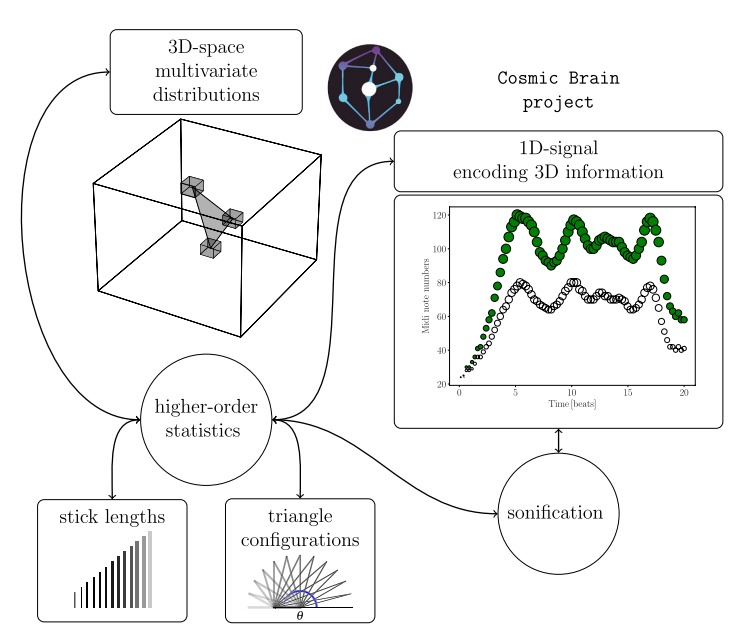
\includegraphics[width=0.8\textwidth]{figures/marco/brain_sonification.jpeg}
    \caption{Diagrama de flujo del proyecto Cosmic Brain, detallando el proceso de codificación de información 3D en una señal 1D para su sonificación. Fuente: Extraído de \cite{Kitaura2025}}
    \label{fig:brain_sonification}
\end{figure}

\subsubsection{Sonificación como alternativa a la navegación}

Otro aspecto importante de la sonificación es que ofrece vias de retroalimentación alternativas. En el trabajo realizado por \cite{Matinfar2023} investigaron la sonificación como una alternativa directa a la navegación quirúrgica visual convencional. Los autores desarrollaron un modelo de cuatro grados de libertad (\textit{4-DOF}) utilizando síntesis de modulación de frecuencia para codificar parámetros espaciales continuos. Los resultados de su estudio revelaron que traducir las métricas de alineación quirúrgica a variaciones acústicas no solo iguala la precisión clínica de las pantallas tradicionales, sino que optimiza la ergonomía cognitiva al evitar que el cirujano deba dividir su atención visual.

\subsubsection{Sonificación como modelo personalizado}
 
La sonificación se ha adaptado para comunicar métricas de salud directamente al paciente. Clark y Doryab \cite{10.1145/3570346} propusieron el uso de modelos musicales personalizados en dispositivos móviles para informar sobre el estado de bienestar del usuario. Su investigación validó que la parametrización de características sonoras, ajustadas a las preferencias individuales, permite transmitir el estado de salud de manera intuitiva y efectiva, abriendo nuevas vías para el diseño de tecnologías orientadas al cambio de comportamiento. En la Figura \ref{fig:features_sonification} se detallan los resultados de esta evaluación, ilustrando la distribución de los puntajes de bienestar (\textit{Health Score}) al ser mapeados a través de cinco dimensiones musicales distintas.

\begin{figure}[H]
    \centering
    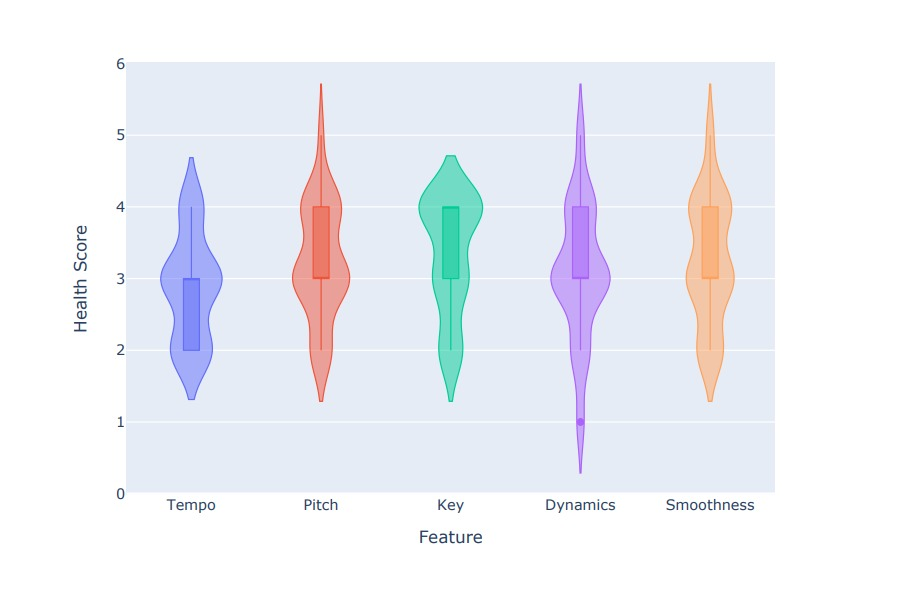
\includegraphics[width=0.8\textwidth]{figures/marco/features_sonification.jpeg}
    \caption{Distribución de puntajes (\textit{Health Score}) para distintas características de la señal acústica: Tempo, Pitch, Key, Dynamics y Smoothness. Fuente: Extraído de \cite{10.1145/3570346}}
    \label{fig:features_sonification}
\end{figure}

\subsubsection{Sonificación de \textit{4D Flow MRI}}

Como un nuevo paso en la aplicación del análisis acústico en el ámbito clínico, este trabajo presenta un modelo de sonificación desarrollado para datos de \textit{4D Flow MRI}. El enfoque principal es abordar la complejidad espacial y temporal de los datos hemodinámicos. Para lograrlo, la metodología extrae las características geométricas y cinemáticas del flujo sanguíneo para mapearlas hacia un modelo de síntesis de audio. Así, al sintetizar acústicamente los datos volumétricos de \textit{4D Flow MRI}, se entrega una nueva forma de análisis sobre estos.